\section{Results}\label{sec:results}

\subsection{Boundary Accuracy}\label{sec:res-f1}
Table~\ref{tab:f1} and Figure~\ref{fig:f1} show boundary F1 scores compared to the gold derived from MorphScore's segmentation into morphemes based on lemmas, for all methods and languages.
Precision and recall scores are in Tables~\ref{tab:precision} and~\ref{tab:recall} of the Appendix, and all methods are shown in precision-recall space in Figure~\ref{fig:pr}.

\begin{table}[!ht]
\centering
\caption{Boundary F1 (\%) compared to MorphScore gold boundaries derived from lemmas, over all unique word forms. Average and standard deviation over 3 training seeds. The best result for each language is in bold.}
\label{tab:f1}
\small
\setlength{\tabcolsep}{4pt}
\begin{tabular}{lccccc}
\toprule
System & English & Spanish & Danish & Tamil & Turkish \\
\midrule
BPE, free marker & 40.0\,{\scriptsize$\pm$1.6} & 18.7\,{\scriptsize$\pm$0.8} & 24.3\,{\scriptsize$\pm$0.8} & 4.4\,{\scriptsize$\pm$2.3} & 35.0\,{\scriptsize$\pm$1.9} \\
POS-weighted BPE & 43.4\,{\scriptsize$\pm$1.6} & 18.9\,{\scriptsize$\pm$0.8} & 24.5\,{\scriptsize$\pm$0.5} & 6.2\,{\scriptsize$\pm$2.3} & 35.0\,{\scriptsize$\pm$1.6} \\
\quad transitions only & 43.4\,{\scriptsize$\pm$1.6} & 18.9\,{\scriptsize$\pm$0.8} & 24.5\,{\scriptsize$\pm$0.5} & 6.2\,{\scriptsize$\pm$2.3} & 35.1\,{\scriptsize$\pm$1.6} \\
\quad penalty only & 42.0\,{\scriptsize$\pm$1.3} & 18.7\,{\scriptsize$\pm$0.8} & 24.4\,{\scriptsize$\pm$1.0} & 4.4\,{\scriptsize$\pm$2.3} & 34.9\,{\scriptsize$\pm$1.9} \\
\addlinespace[2pt]
Content-word-weighted BPE & 43.9\,{\scriptsize$\pm$0.2} & 16.5\,{\scriptsize$\pm$0.3} & 27.8\,{\scriptsize$\pm$0.7} & 22.2\,{\scriptsize$\pm$1.1} & 34.2\,{\scriptsize$\pm$0.4} \\
Lemma2Word + BPE & \textbf{59.9\,{\scriptsize$\pm$0.1}} & \textbf{36.3\,{\scriptsize$\pm$0.1}} & \textbf{43.8\,{\scriptsize$\pm$0.3}} & \textbf{52.9\,{\scriptsize$\pm$0.4}} & \textbf{48.7\,{\scriptsize$\pm$0.1}} \\
BPE, word-initial marker & 25.5\,{\scriptsize$\pm$0.4} & 6.7\,{\scriptsize$\pm$0.5} & 13.1\,{\scriptsize$\pm$0.1} & 7.5\,{\scriptsize$\pm$0.3} & 40.8\,{\scriptsize$\pm$0.4} \\
Unigram LM & 54.3\,{\scriptsize$\pm$0.5} & 29.0\,{\scriptsize$\pm$0.0} & 35.1\,{\scriptsize$\pm$0.5} & 43.0\,{\scriptsize$\pm$0.8} & 46.5\,{\scriptsize$\pm$0.4} \\
\bottomrule
\end{tabular}
\end{table}


\begin{figure}[!ht]
\centering
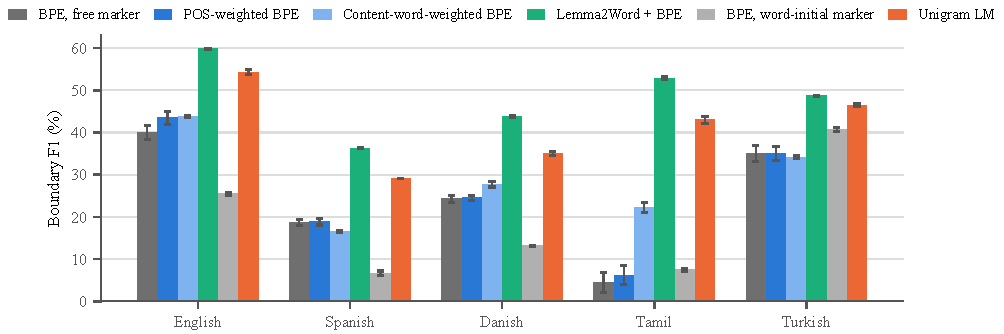
\includegraphics[width=\linewidth]{figures/fig_f1.pdf}
\caption{Boundary F1 (\%) for the six main tokenizers, over 5 languages. The bars show the average over 3 training seeds, and error bars one standard deviation.}
\label{fig:f1}
\end{figure}

The results in Table~\ref{tab:f1} also show that Lemma2Word (Section~\ref{sec:l2w}) offers the best F1 score in all languages, with a range from \nFLtwSpanish\% in Spanish to \nFLtwEnglish\% in English.
The unigram model is in second place in all languages, and leads all BPE variants by a wide margin in Tamil (F1 of \nFUniTamil{} vs.\ \nFBpeTamil).
POS-weighted BPE differs from its unweighted base by about three percentage points in English (\nFPosEnglish\% vs.\ \nFBpeEnglish\%) and by less than a point in Spanish, Danish, and Turkish.
The difference in English is the only one bigger than the variation due to random seeds.
Ablation experiments also show that the transition term alone accounts for the improvement; a version using only the transition term produces the same F1 score as the full model while a version using only the penalty term performs the same as the unweighted base model.

The F1 score using content-word weighting (Section~\ref{sec:content}) increases over plain BPE from \nFBpeTamil\% to \nFPosContentTamil\% in Tamil and by about three percentage points in English and Danish, but decreases in Spanish and Turkish.
The variant with a word-initial marker (Section~\ref{sec:freebpe}), following the SentencePiece standard, produces the worst scores in four languages because the whole word plus the marker is a single token and thus has fewer word boundaries inserted than the variant with a free marker; in Spanish for example its recall is only \nRHfBpeSpanish\% vs.\ \nRBpeSpanish\% for the free marker variant.

Figure~\ref{fig:pr} shows boundary precision versus recall for each language (points indicate the mean over the three seeds, error bars show one standard deviation, and most are smaller than the markers).

\begin{figure}[!ht]
\centering
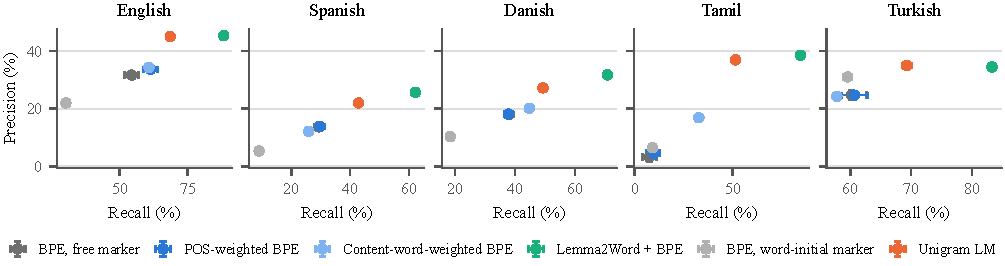
\includegraphics[width=\linewidth]{figures/fig_pr.pdf}
\caption{Boundary precision against recall per language. Points are means over three seeds and error bars span one standard deviation; most are smaller than the markers.}
\label{fig:pr}
\end{figure}

\subsection{What the Part-of-Speech Weighting Changes}\label{sec:res-pos}
The weight in Section~\ref{sec:posbpe} affects merges only at the right word boundaries, i.e.\ when a word is merged with the following space.
The effect of these merges is measured on held-out text in Table~\ref{tab:span}.
Plain free-marker BPE puts word boundaries inside tokens in \nSpanShareBpeTurkish\% to \nSpanShareBpeSpanish\% of cases (for Turkish and Spanish respectively), while the POS weighting does not change this proportion much in most languages, but reduces it from \nSpanShareBpeTamil{} to \nSpanSharePosTamil{} in Tamil\footnote{Seed 0; the three-seed mean of the share of tokens that span a boundary falls from \nCrossBpeTamil\% to \nCrossPosTamil\% (Table~\ref{tab:cross}).}.
The transitions spanned are the same ones BPE spans: in English, for example, cases of an adposition before a determiner (\texttt{of\textvisiblespace the\textvisiblespace}), in Spanish cases of determiner before noun, in Danish cases of noun before adposition.

Across all languages, variants, and with or without weighting, the mean transition probability at a spanned boundary is no more than two percentage points away from the mean over all boundaries.
The proportion of tokens crossing boundaries depends on how often each type of boundary occurs.
The transition probabilities are no more than frequencies of tag pairs and carry no additional information beyond the counts of symbols.

\begin{table}[!ht]
\centering
\caption{Percentage of word boundaries spanned by a token in held-out text, mean probability (\%) of the POS transition at spanned boundaries, and the same mean over all boundaries. Results are from seed 0; the most common spanned transition and token are shown for the POS-weighted model.}
\label{tab:span}
\footnotesize
\setlength{\tabcolsep}{3.5pt}
\begin{tabular}{llccclc}
\toprule
Language & System & spanned (\%) & $P$, spanned & $P$, all & top transition & top token \\
\midrule
English & BPE, free marker & 45.2 & 23.3 & 22.1 & ADP$\to$DET & \texttt{in\textvisiblespace{}the\textvisiblespace{}} \\
 & POS-weighted BPE & 42.6 & 23.5 & 22.1 & ADP$\to$DET & \texttt{of\textvisiblespace{}the\textvisiblespace{}} \\
 & Content-word-weighted BPE & 33.2 & 24.4 & 22.1 & ADP$\to$DET & \texttt{of\textvisiblespace{}the\textvisiblespace{}} \\
\addlinespace[2pt]
Spanish & BPE, free marker & 54.1 & 32.3 & 28.2 & DET$\to$NOUN & \texttt{a\textvisiblespace{}de\textvisiblespace{}} \\
 & POS-weighted BPE & 54.1 & 32.3 & 28.2 & DET$\to$NOUN & \texttt{a\textvisiblespace{}de\textvisiblespace{}} \\
 & Content-word-weighted BPE & 43.5 & 33.8 & 28.2 & DET$\to$NOUN & \texttt{en\textvisiblespace{}la\textvisiblespace{}} \\
\addlinespace[2pt]
Danish & BPE, free marker & 41.3 & 21.1 & 22.4 & NOUN$\to$ADP & \texttt{en\textvisiblespace{}i\textvisiblespace{}} \\
 & POS-weighted BPE & 41.4 & 21.1 & 22.4 & NOUN$\to$ADP & \texttt{en\textvisiblespace{}i\textvisiblespace{}} \\
 & Content-word-weighted BPE & 31.0 & 20.9 & 22.4 & NOUN$\to$ADP & \texttt{er\textvisiblespace{}i\textvisiblespace{}} \\
\addlinespace[2pt]
Tamil & BPE, free marker & 54.1 & 24.4 & 24.9 & NOUN$\to$NOUN & \tamil{ு}\textvisiblespace{}\tamil{ப} \\
 & POS-weighted BPE & 39.5 & 25.0 & 24.9 & NOUN$\to$NOUN & \tamil{ு}\textvisiblespace{}\tamil{ப} \\
 & Content-word-weighted BPE & 7.4 & 26.5 & 24.9 & NOUN$\to$NOUN & \tamil{ப்}\textvisiblespace{}\tamil{ப} \\
\addlinespace[2pt]
Turkish & BPE, free marker & 15.5 & 22.3 & 25.0 & NOUN$\to$CCONJ & \texttt{i\textvisiblespace{}ve\textvisiblespace{}} \\
 & POS-weighted BPE & 15.2 & 22.5 & 25.0 & NOUN$\to$CCONJ & \texttt{i\textvisiblespace{}ve\textvisiblespace{}} \\
 & Content-word-weighted BPE & 9.0 & 23.7 & 25.0 & NOUN$\to$CCONJ & \texttt{i\textvisiblespace{}ve\textvisiblespace{}} \\
\addlinespace[2pt]
\bottomrule
\end{tabular}
\end{table}


\subsection{Content-Word Weighting}\label{sec:res-content}
Doubling the weight in Section~\ref{sec:content} on merges inside some POS categories (nouns, proper nouns, verbs, adjectives) is meant to spend more of the vocabulary budget on complete content words.
That results in various benefits and drawbacks, depending on the language.
First, it decreases the percentage of cases in which a token spans a boundary in all languages (Table~\ref{tab:cross}), while in Tamil for example the recall increases from \nRBpeTamil{} to \nRPosContentTamil{} (plain BPE hardly cuts at the stem boundary).
In Spanish and Turkish however it decreases recall because whole-word tokens take the place of suffix tokens that plain BPE learns.
The weight of 2 was not tuned; varying it would make it a tuned method, which we did not do.

\subsection{Lemma2Word}\label{sec:res-l2w}
Table~\ref{tab:l2w} distinguishes between the variant that uses only learned boundaries (the lexicon variant) and the variant that lemmatizes each word on the fly using Stanza (the online variant).
All forms, forms not in training text, and UD test split forms are also reported separately.

\begin{table}[!ht]
\centering
\caption{Boundary recall and precision (\%) in Lemma2Word, by subset of words and variant. The lexicon variant uses only learned boundaries and affixes, the online variant lemmatizes the word to be tokenized with Stanza. Results averaged over three random seeds.}
\label{tab:l2w}
\small
\setlength{\tabcolsep}{3.5pt}
\begin{tabular}{llcccccc}
\toprule
 & & \multicolumn{2}{c}{all} & \multicolumn{2}{c}{unseen} & \multicolumn{2}{c}{UD test} \\
\cmidrule(lr){3-4}\cmidrule(lr){5-6}\cmidrule(lr){7-8}
Language & Variant & R & P & R & P & R & P \\
\midrule
English & lexicon & 88.2 & 45.3 & 73.7 & 30.3 & 84.0 & 37.2 \\
 & online & 98.2 & 50.9 & 98.2 & 41.1 & 91.1 & 40.9 \\
 & BPE, free marker & 54.4 & 31.6 & 54.5 & 25.5 & 49.2 & 24.8 \\
\addlinespace[2pt]
Spanish & lexicon & 62.2 & 25.6 & 40.2 & 15.3 & 48.1 & 18.3 \\
 & online & 99.1 & 39.0 & 99.1 & 35.4 & 94.8 & 34.2 \\
 & BPE, free marker & 29.4 & 13.7 & 35.8 & 14.7 & 31.8 & 13.2 \\
\addlinespace[2pt]
Danish & lexicon & 70.8 & 31.7 & 49.5 & 17.9 & 65.5 & 27.2 \\
 & online & 97.2 & 43.6 & 97.1 & 35.3 & 88.0 & 37.0 \\
 & BPE, free marker & 37.9 & 17.9 & 41.0 & 15.9 & 38.0 & 16.7 \\
\addlinespace[2pt]
Tamil & lexicon & 84.5 & 38.5 & 74.2 & 27.4 & 80.6 & 34.7 \\
 & online & 97.6 & 46.3 & 97.7 & 38.5 & 91.5 & 39.9 \\
 & BPE, free marker & 7.4 & 3.2 & 7.0 & 2.5 & 5.9 & 2.4 \\
\addlinespace[2pt]
Turkish & lexicon & 83.3 & 34.4 & 81.7 & 31.2 & 82.7 & 32.0 \\
 & online & 88.6 & 37.6 & 88.4 & 34.8 & 89.1 & 35.6 \\
 & BPE, free marker & 60.2 & 24.7 & 60.5 & 23.2 & 60.4 & 23.2 \\
\addlinespace[2pt]
\bottomrule
\end{tabular}
\end{table}


The lexicon variant has a major improvement over the unweighted BPE in recall, from \nRBpeEnglish{} to \nLtwLexiconAllREnglish{} percent in English and \nRBpeTamil{} to \nLtwLexiconAllRTamil{} percent in Tamil, and 23--34 percentage points for the other three languages.
Precision is improved as well, since BPE on the shorter pieces learns fewer internal boundaries.
The 20-occurrence threshold also admits fewer of the short and ambiguous inflectional suffixes of Spanish and Danish in combinations of word-final letter sequences.
In terms of unseen forms, recall is \nLtwLexiconUnseenREnglish{} percent in English, \nLtwLexiconUnseenRTamil{} in Tamil, and falls to a few points in Spanish and Danish for the short and ambiguous word-final letter sequences.

The online variant recovers nearly all the correct boundaries, reaching \nLtwOnlineAllRSpanish{} percent recall in Spanish because the gold boundaries were extracted from the lemmas, and the lemmatizer could recall the correct lemma from its memory on the training data.
On the UD test-split forms, which the lemmatizer never saw, recall drops, but is still within \nLtwOnlineTestRDanish--\nLtwOnlineTestRSpanish{} percent.
Its precision, however, is no better than 51 percent, because the BPE can still split inside the input pieces, while the gold standard marks only the boundaries around the word stem.

\subsection{Compression and Stability}\label{sec:res-compression}
Table~\ref{tab:tpw} reports the average tokenization efficiency, measured as the average number of tokens produced per word, on the held-out text.
The effect of the POS weighting on compression is less than one percent.
In English, Lemma2Word produces \nTpwLtwEnglish{} tokens per word compared to \nTpwBpeEnglish{} for the free-marker BPE, an increase of four percent.
In Spanish the increase is larger, eight percent, with Lemma2Word producing \nTpwLtwSpanish{} tokens per word compared to \nTpwBpeSpanish{} for the free-marker BPE.
Lemma2Word is more compact than the unigram model for all languages except Tamil.
The tokenizers that are provided as reference never cross a word boundary, and are more expensive in terms of tokens per word in the three European languages, and cheaper in the two others (Tamil, Turkish), because the free-marker BPE budget in these two languages is partly spent on tokens that cover frequent word pairs.

\begin{table}[!ht]
\centering
\caption{Tokens per whitespace word on held-out Wikipedia paragraphs (lower is more compact).}
\label{tab:tpw}
\small
\setlength{\tabcolsep}{4pt}
\begin{tabular}{lccccc}
\toprule
System & English & Spanish & Danish & Tamil & Turkish \\
\midrule
BPE, free marker & 1.481\,{\scriptsize$\pm$0.002} & 1.413\,{\scriptsize$\pm$0.002} & 1.606\,{\scriptsize$\pm$0.002} & 2.242\,{\scriptsize$\pm$0.005} & 1.962\,{\scriptsize$\pm$0.002} \\
POS-weighted BPE & 1.470\,{\scriptsize$\pm$0.001} & \textbf{1.412\,{\scriptsize$\pm$0.001}} & \textbf{1.604\,{\scriptsize$\pm$0.002}} & 2.215\,{\scriptsize$\pm$0.006} & 1.938\,{\scriptsize$\pm$0.025} \\
\quad transitions only & 1.470\,{\scriptsize$\pm$0.001} & 1.412\,{\scriptsize$\pm$0.001} & 1.604\,{\scriptsize$\pm$0.002} & 2.215\,{\scriptsize$\pm$0.006} & 1.938\,{\scriptsize$\pm$0.025} \\
\quad penalty only & \textbf{1.470\,{\scriptsize$\pm$0.001}} & 1.413\,{\scriptsize$\pm$0.002} & 1.605\,{\scriptsize$\pm$0.002} & 2.243\,{\scriptsize$\pm$0.005} & 1.962\,{\scriptsize$\pm$0.003} \\
\addlinespace[2pt]
Content-word-weighted BPE & 1.486\,{\scriptsize$\pm$0.002} & 1.423\,{\scriptsize$\pm$0.002} & 1.619\,{\scriptsize$\pm$0.001} & 2.150\,{\scriptsize$\pm$0.012} & 1.998\,{\scriptsize$\pm$0.003} \\
Lemma2Word + BPE & 1.538\,{\scriptsize$\pm$0.001} & 1.531\,{\scriptsize$\pm$0.002} & 1.703\,{\scriptsize$\pm$0.001} & 2.376\,{\scriptsize$\pm$0.002} & 2.080\,{\scriptsize$\pm$0.010} \\
BPE, word-initial marker & 1.555\,{\scriptsize$\pm$0.001} & 1.565\,{\scriptsize$\pm$0.000} & 1.713\,{\scriptsize$\pm$0.001} & \textbf{2.042\,{\scriptsize$\pm$0.001}} & \textbf{1.883\,{\scriptsize$\pm$0.002}} \\
Unigram LM & 1.609\,{\scriptsize$\pm$0.001} & 1.607\,{\scriptsize$\pm$0.002} & 1.778\,{\scriptsize$\pm$0.004} & 2.177\,{\scriptsize$\pm$0.006} & 2.004\,{\scriptsize$\pm$0.004} \\
\bottomrule
\end{tabular}
\end{table}


The reliability is measured in the appendices (Tables~\ref{tab:jaccard} and~\ref{tab:agreement}) by comparing the vocabularies produced on different training samples, and the segmentations of the same held-out text produced by different models trained on different samples using the same method.
In both cases, the reliability statistics are far less discriminative than accuracy.
The Jaccard measure of the vocabularies shows a range of 62--79 percent overlap in entries for vocabularies produced from different training samples; the segmentations produced by the same method show a range of 88--97 percent agreement.
The POS weighting does not improve these statistics, and for the overlap in the Turkish vocabulary the POS weighting is actually a detriment, going from \nJacBpeTurkish{} to \nJacPosTurkish{} percent, with a standard deviation of \nJacPosTurkishSd{} percentage points, the least stable of the cases shown in the table.
The unigram model has the lowest vocabulary overlap in all languages and the same range of agreement as all the other methods, and the difference in the vocabularies produced from the unigram model is restricted mostly to rare entries that are unlikely to be seen in the held-out text.

\subsection{Vocabulary Budget}\label{sec:res-sweep}
Comparing the performance of the different methods at two other vocabulary budgets (2,000 and 32,000 types) in Figure~\ref{fig:sweep}, the relative ranking of the methods is maintained at all budgets.
Lemma2Word improves with larger vocabularies, moving up from \nSweepFLtwEnglishVTwoK{} to \nSweepFLtwEnglishVThirtyTwoK{} percent F1 in English, for example, due to the larger budget allowing more word pieces to remain unsplit.
The unigram model moves down at 32,000 types in English, Tamil, and Turkish, where the budget exceeds what a 3,000-paragraph sample can support and whole words enter the vocabulary.
The difference between the POS-weighted BPE and the unweighted BPE is less than three percentage points at all budget sizes.

\begin{figure}[!ht]
\centering
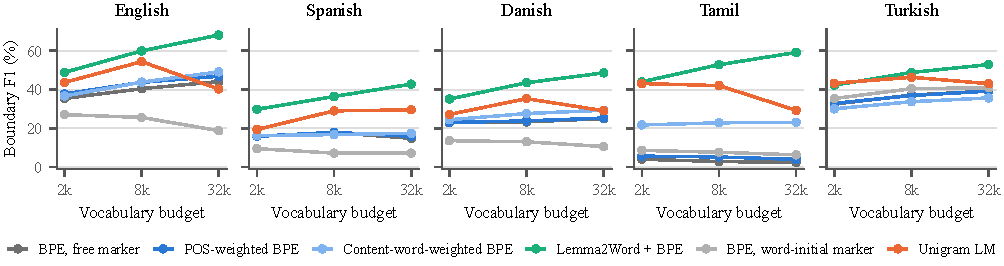
\includegraphics[width=\linewidth]{figures/fig_sweep.pdf}
\caption{Boundary F1 (\%) at vocabulary budgets of 2,000, 8,000, and 32,000 types using seed 0.}
\label{fig:sweep}
\end{figure}

\subsection{Language-Model Probe}\label{sec:res-lm}
Table~\ref{tab:bpc} reports the bits per character of the language model trained on the different tokenizers, and Figure~\ref{fig:bpc} shows the same data graphically.
A language model is trained for each tokenizer seed, and across these different seeds the standard deviation is less than 0.01 bits in most cases, and never more than 0.03 bits.
Differences of a few hundredths of a bit can therefore be considered reliable at this scale.

\begin{table}[!ht]
\centering
\caption{Bits per character in the language model trained on the output of the tokenizer. The language model has 7M parameters and is trained for 6 passes over the same text with each tokenizer. Lower scores are better, and we show the mean and one standard deviation for the three tokenizer seeds.}
\label{tab:bpc}
\small
\setlength{\tabcolsep}{4pt}
\begin{tabular}{lccccc}
\toprule
System & English & Spanish & Danish & Tamil & Turkish \\
\midrule
BPE, free marker & 2.807\,{\scriptsize$\pm$0.002} & 2.689\,{\scriptsize$\pm$0.003} & 2.878\,{\scriptsize$\pm$0.001} & 2.848\,{\scriptsize$\pm$0.006} & 2.963\,{\scriptsize$\pm$0.002} \\
POS-weighted BPE & 2.785\,{\scriptsize$\pm$0.001} & 2.687\,{\scriptsize$\pm$0.001} & 2.874\,{\scriptsize$\pm$0.001} & 2.819\,{\scriptsize$\pm$0.005} & 2.935\,{\scriptsize$\pm$0.032} \\
\quad transitions only & 2.785\,{\scriptsize$\pm$0.001} & 2.687\,{\scriptsize$\pm$0.001} & 2.874\,{\scriptsize$\pm$0.002} & 2.819\,{\scriptsize$\pm$0.005} & 2.935\,{\scriptsize$\pm$0.032} \\
\quad penalty only & 2.786\,{\scriptsize$\pm$0.002} & 2.689\,{\scriptsize$\pm$0.002} & 2.876\,{\scriptsize$\pm$0.001} & 2.849\,{\scriptsize$\pm$0.006} & 2.963\,{\scriptsize$\pm$0.003} \\
\addlinespace[2pt]
Content-word-weighted BPE & 2.794\,{\scriptsize$\pm$0.001} & 2.680\,{\scriptsize$\pm$0.003} & 2.868\,{\scriptsize$\pm$0.001} & 2.737\,{\scriptsize$\pm$0.015} & 2.995\,{\scriptsize$\pm$0.003} \\
Lemma2Word + BPE & 2.887\,{\scriptsize$\pm$0.003} & 2.861\,{\scriptsize$\pm$0.004} & 3.007\,{\scriptsize$\pm$0.001} & 2.983\,{\scriptsize$\pm$0.002} & 3.096\,{\scriptsize$\pm$0.011} \\
BPE, word-initial marker & 2.715\,{\scriptsize$\pm$0.003} & 2.674\,{\scriptsize$\pm$0.006} & 2.909\,{\scriptsize$\pm$0.003} & 2.611\,{\scriptsize$\pm$0.001} & 2.808\,{\scriptsize$\pm$0.004} \\
Unigram LM & \textbf{2.531\,{\scriptsize$\pm$0.006}} & \textbf{2.473\,{\scriptsize$\pm$0.011}} & \textbf{2.704\,{\scriptsize$\pm$0.007}} & \textbf{2.524\,{\scriptsize$\pm$0.003}} & \textbf{2.694\,{\scriptsize$\pm$0.003}} \\
\bottomrule
\end{tabular}
\end{table}


\begin{figure}[!ht]
\centering
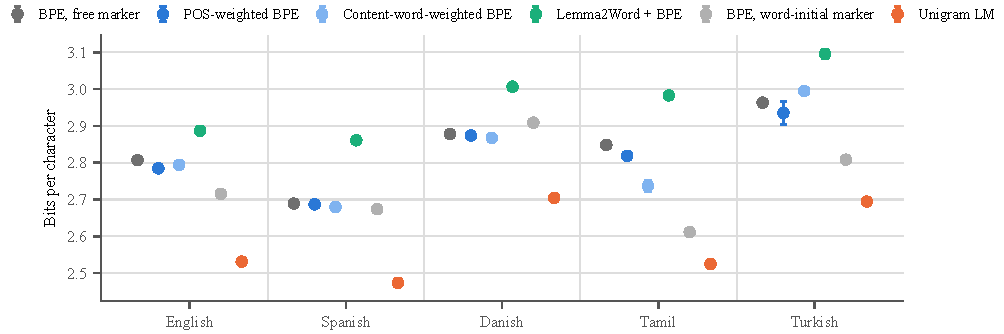
\includegraphics[width=\linewidth]{figures/fig_bpc.pdf}
\caption{Bits per character in the language model trained on the output of the tokenizer. The language model has 7M parameters and is trained for 6 passes over the same text with each tokenizer. Lower scores are better, and we show the mean and one standard deviation for the three tokenizer seeds. The y-axis starts at 2.4 bits to show the differences.}
\label{fig:bpc}
\end{figure}

However, the ordering by bits-per-character does not match the ordering by boundary-F1.
The unigram model has been ranked second by F1 and first by bits-per-character in all languages.
In English it is first with \nBpcUniEnglish{} bits-per-character compared to \nBpcBpeEnglish{} for free-marker BPE.
In Tamil the first place is taken by the unigram model with \nBpcUniTamil{} bits compared to \nBpcBpeTamil{} for free-marker BPE.
Lemma2Word has been ranked first by F1 and last by bits-per-character in all languages.
In English Lemma2Word is ranked last with \nBpcLtwEnglish{} bits-per-character.
The word cutting using stem boundaries before training the subword tokenizer is removing frequent full-word tokens and adding tokens that are too unpredictable for a model of this size to compensate.

Word-initial BPE has been ranked last by F1 in four languages.
In four languages, it has been ranked ahead of free-marker BPE by bits-per-character.
In English it is ranked ahead with \nBpcHfBpeEnglish{} vs.\ \nBpcBpeEnglish.
The tokens crossing word boundaries, which help compactness in free-marker BPE, do not help in prediction.
POS weighting has been changing bits-per-character by less than 0.03 in all the languages, so it seems it is pointing in a positive direction but with a small contribution.
Interestingly, the table shows that for Turkish the seed-to-seed variation in bits-per-character is the highest.
The two ablations with POS weighting give the same result.
Content word weighting has been reducing bits-per-character in Tamil to \nBpcPosContentTamil{} vs.\ \nBpcBpeTamil.
This was also the language where it has been giving the largest improvement in boundary-F1.
On the other hand, in Turkish content-word weighting has been increasing the bits-per-character numbers.

Since all the tokenizers are trained on the same text, the number of passes is the same for all models; they go over the data 6 times.
Since a higher token count therefore leads to more optimizer steps, the unigram model has 8.6\% more optimizer steps than free-marker BPE in English.
To control for the change in optimizer steps, we have trained a model for free-marker BPE in seed 0 with 10\% fewer optimizer steps (5.4 passes over the data) and 10\% more optimizer steps (6.6 passes).
The bits-per-character changes from \nBpcControlBase{} to \nBpcControlLow{} and \nBpcControlHigh{} respectively.
These changes are small compared to the ones between tokenizers, so the step count cannot be used to explain the model ranking.
Since Lemma2Word has a higher number of tokens than free-marker BPE and it has been ranked behind, the reason cannot be the optimizer step count alone.

These results indicate that morphological alignment and the quality of the model do not move together at this scale, which agrees with the conclusions reached about the unigram model by \citet{bostrom2020bpe}.
This also supports the finding that the intrinsic measures for tokenizers are not perfect predictors for downstream tasks~\cite{ali2024tokenizer,schmidt2024tokenization}.

\subsection{A Language Model as a Segmenter}\label{sec:res-llm}
Table~\ref{tab:llm} shows the results of the study described in Section~\ref{sec:llm}.
For each language, a sample of 400 word forms were randomly selected from the gold standard list using seed 0.
The Claude Sonnet model (\texttt{claude-sonnet-5-5}, October 2026 version) was selected and it was prompted to add plus signs between morphemes in batches of 40 words.
The prompt used does not allow any character modification and is given in Appendix~\ref{app:prompt}.
Answers that change the characters of the word are invalid and they were not counted when computing the scores.
To compare with the same seed 0 tokenizers, we have evaluated them on the same words that the model had given valid answers for.

\begin{table}[!ht]
\centering
\caption{Claude Sonnet segmenting words into morphemes, on a fixed random sample of gold standard forms. The seed 0 tokenizers are evaluated on the same words. Invalid answers are answers that change the characters of the word and they were not counted in the computation of the scores. The table reports boundary precision, recall and F1 (in \%), and the number of tokens per word after segmentation.}
\label{tab:llm}
\small
\setlength{\tabcolsep}{3.5pt}
\begin{tabular}{lrrcccccccc}
\toprule
 & & & \multicolumn{4}{c}{language model} & \multicolumn{3}{c}{recall of tokenizers on the same words} \\
\cmidrule(lr){4-7}\cmidrule(lr){8-10}
Language & words & invalid & P & R & F1 & pieces/word & Lemma2Word & Unigram & BPE, free \\
\midrule
English & 400 & 0 & 77.6 & 91.0 & 83.8 & 2.17 & 87.0 & 69.2 & 52.2 \\
Spanish & 399 & 1 & 35.1 & 69.9 & 46.8 & 2.99 & 62.2 & 44.1 & 25.3 \\
Danish & 400 & 0 & 38.9 & 66.0 & 49.0 & 2.69 & 72.5 & 50.0 & 42.0 \\
Tamil & 393 & 7 & 72.6 & 90.4 & 80.5 & 2.25 & 84.8 & 48.9 & 6.8 \\
Turkish & 400 & 0 & 50.7 & 96.5 & 66.5 & 2.90 & 84.8 & 67.2 & 60.2 \\
\bottomrule
\end{tabular}
\end{table}


The model has been able to surpass the recall on gold boundaries of any of the tokenizers in four languages.
In English the model gets \nLlmREnglish\% compared to \nLlmSampleLtwREnglish\% for Lemma2Word, in Tamil \nLlmRTamil\% vs.\ \nLlmSampleLtwRTamil\% and in Turkish \nLlmRTurkish\% vs.\ \nLlmSampleLtwRTurkish\%.
The model has been ranked behind Lemma2Word in Danish with \nLlmRDanish\% recall vs.\ \nLlmSampleLtwRDanish\%.
The precision of the model is ranging between \nLlmPSpanish\% and \nLlmPEnglish\%.
The model marks derivational affixes and parts of compounds that are not included in the lemma-based gold standard, and the number of pieces per word is between \nLlmTpwEnglish{} and \nLlmTpwSpanish{} compared to the maximum of 3 pieces per word in the gold.
Almost all of the answers preserve the characters of the words in the Latin script, and there was only \nLlmInvalidSpanish{} invalid answer for Spanish and none for the other Latin-script languages.

Tamil had two issues.
The model had long reasoning chains, the 40-word batches exceeded the response length, and the unanswered words had to be re-asked in 15-word batches.
The model had also written the underlying morphemes in \nLlmInvalidTamil{} answers rather than the surface forms, violating the character constraint.
In one of them the model gave \tamil{கள்}\,+\,\tamil{உக்கு} instead of \tamil{களுக்கு}, since the suffix vowel fuses with the consonant.
The study used approximately 2,000 words and the cost of the API was minimal (a few dollars).
This evaluation is not showing what a tokenizer built on top of the model's responses would be capable of, but what the model knows about the morphology.
The answers from the model do not have a fixed vocabulary and they are not guaranteed to be in a consistent format even if the same word occurs multiple times.
The cost per word is several orders of magnitude more than any of the tokenizers shown in Table~\ref{tab:f1}.
The answers could be used off-line to generate a segmentation lexicon similar to the output of Lemma2Word to provide boundaries in places where a lemmatizer doesn't exist.
This use case is not evaluated in the paper.

